\documentclass[11pt, letterpaper,oneside]{article}
\usepackage[utf8]{inputenc}
\usepackage{multirow}
\usepackage{physics}
\usepackage{float}
\usepackage{amsfonts}
\usepackage{graphicx}
\usepackage[english]{babel}
\usepackage{hyperref}

\title{East-West Method Analysis over All Triggers Dataset}
\author{E.Coronel\footnote{evelyn.coronel@ib.edu.ar},  S. Mollerach}
\date{February 2021}

\begin{document}

\begin{titlepage}
\maketitle
\end{titlepage}


\begin{table}[H]
    \begin{small}
        \begin{center}
            \begin{tabular}{lc|l|l|l|}
\hline
\multicolumn{1}{|l|}{\multirow{4}{*}{\begin{tabular}[c]{@{}c@{}}Rango \\ Tiempo\end{tabular}}}    & Todos       & Inicio &\multicolumn{2}{l|}{1 de Enero, 2014 } \\ \cline{3-5} 
\multicolumn{1}{|l|}{}                                                                            & 6 años      & Fin    &\multicolumn{2}{l|}{1 de Enero, 2020} \\ \cline{2-5} 
\multicolumn{1}{|l|}{}                                                                            & Estándar    & Inicio &\multicolumn{2}{l|}{1 de Enero, 2004} \\ \cline{3-5}
\multicolumn{1}{|l|}{}                                                                            & 14.7 años   & Fin    &\multicolumn{2}{l|}{1 de Agosto, 2018} \\ \hline  \\

\hline                                                                          \multicolumn{2}{|c|}{Rango [EeV]}                                                    & \multicolumn{1}{c|}{0.25 - 0.5}  & \multicolumn{1}{c|}{ 0.5  - 1 } &\multicolumn{1}{c|}{ 1 - 2 } \\ \hline
\multicolumn{1}{|l|}{\multirow{2}{*}{Eventos}}                            & Todos    & $3\,967\,368$     & $3\,638\,226$   & $1\,081\,846$ \\ \cline{2-5} 
\multicolumn{1}{|l|}{}                                                    & Estándar & $770\,316$        & $2\,388\,467$   & $1\,243\,103$ \\ \hline
\multicolumn{1}{|l|}{\multirow{2}{*}{\begin{tabular}[c]{@{}c@{}}Energía \\ Media\end{tabular}}} & Todos    & $0.38$           & $0.69$         & $1.32$       \\ \cline{2-5} 
\multicolumn{1}{|l|}{}                                                                             & Estándar & $0.43$            & $0.70$          & $1.28$       \\ \hline
\end{tabular}
            \caption{Características de los conjuntos de datos para distintos rangos de energía }
            \label{tab:datasets}
        \end{center}
    \end{small}
\end{table}


\section{Resultados en distintos rangos de energía}
\subsection{Results of the 0.25 EeV - 0.5 EeV energy range}



\begin{table}[H]
    \begin{small}
        \begin{center}
            \begin{tabular}[c]{l|c|c||c|}
\cline{2-4}                                       & \multicolumn{2}{c||}{All Triggers}    & \multicolumn{1}{c|}{Disparo Estándar}   \\ \hline
\multicolumn{1}{|l|}{Frecuencia:                } & Solar	                & Sidérea	                & Sidérea \cite{Aab_2020}   \\ \hline
\multicolumn{1}{|l|}{Amplitude r [\%]:           } & $0.17^{+0.22}_{-0.07}$	& $0.12^{+0.24}_{-0.03}$ 	& $0.5^{+0.4}_{-0.2}$ \cite{codigo}      \\
\multicolumn{1}{|l|}{$r_{99}$ [\%]:             } & \multicolumn{2}{c||}{0.58}                          & 1.1\cite{codigo}                 \\
\multicolumn{1}{|l|}{$r^{UL}$ [\%]:             } & 0.67 	                & 0.64                      & 1.4\cite{codigo}                 \\ 
\multicolumn{1}{|l|}{$\sigma$[\%]:              } & \multicolumn{2}{c||}{0.19}                          & 0.38\cite{codigo}       \\\hline
\multicolumn{1}{|l|}{Amplitude $d_\perp$[\%]:    } & -	                    & $0.16^{+0.31}_{-0.04}$ 	& $0.6^{+0.5}_{-0.3}$       \\
\multicolumn{1}{|l|}{$d_{99}$ [\%]:             } & - 	                    & 0.73                      & 1.5  \cite{codigo}                \\
\multicolumn{1}{|l|}{$d_{\perp}^{UL}[\%]$       } & -                       & 0.80                      & 1.8                         \\
\multicolumn{1}{|l|}{$\sigma_{x,y}$[\%]:        } & -	                    & 0.24	                    & 0.48       \\\hline
\multicolumn{1}{|l|}{Rayleigh Probability      :        } & 0.66                    & 0.81	                    & 0.45       \\
\multicolumn{1}{|l|}{Phase[$^o$]:                } & 221$\pm$77              & 280$\pm$90                & 225$\pm$64\\ \hline
\multicolumn{1}{|l|}{$\langle\cos\delta \rangle$} & \multicolumn{2}{c||}{0.79}        	                & 0.79 \cite{codigo}        \\        
\multicolumn{1}{|l|}{$\langle\sin\theta \rangle$} & \multicolumn{2}{c||}{0.46}        	                & 0.52 \cite{codigo}        \\ \hline       
            \end{tabular}
            
        \end{center}
    \end{small}
    \caption{Características para las frecuencias solar y sidérea con el método East-West en el primer armónico en rango de energía 0.25 EeV - 0.5 EeV.}
    \label{tab:primer_bin_data}
\end{table}

\begin{figure}[H]
    \begin{small}
        \begin{center}
            \vspace*{-1. cm}
            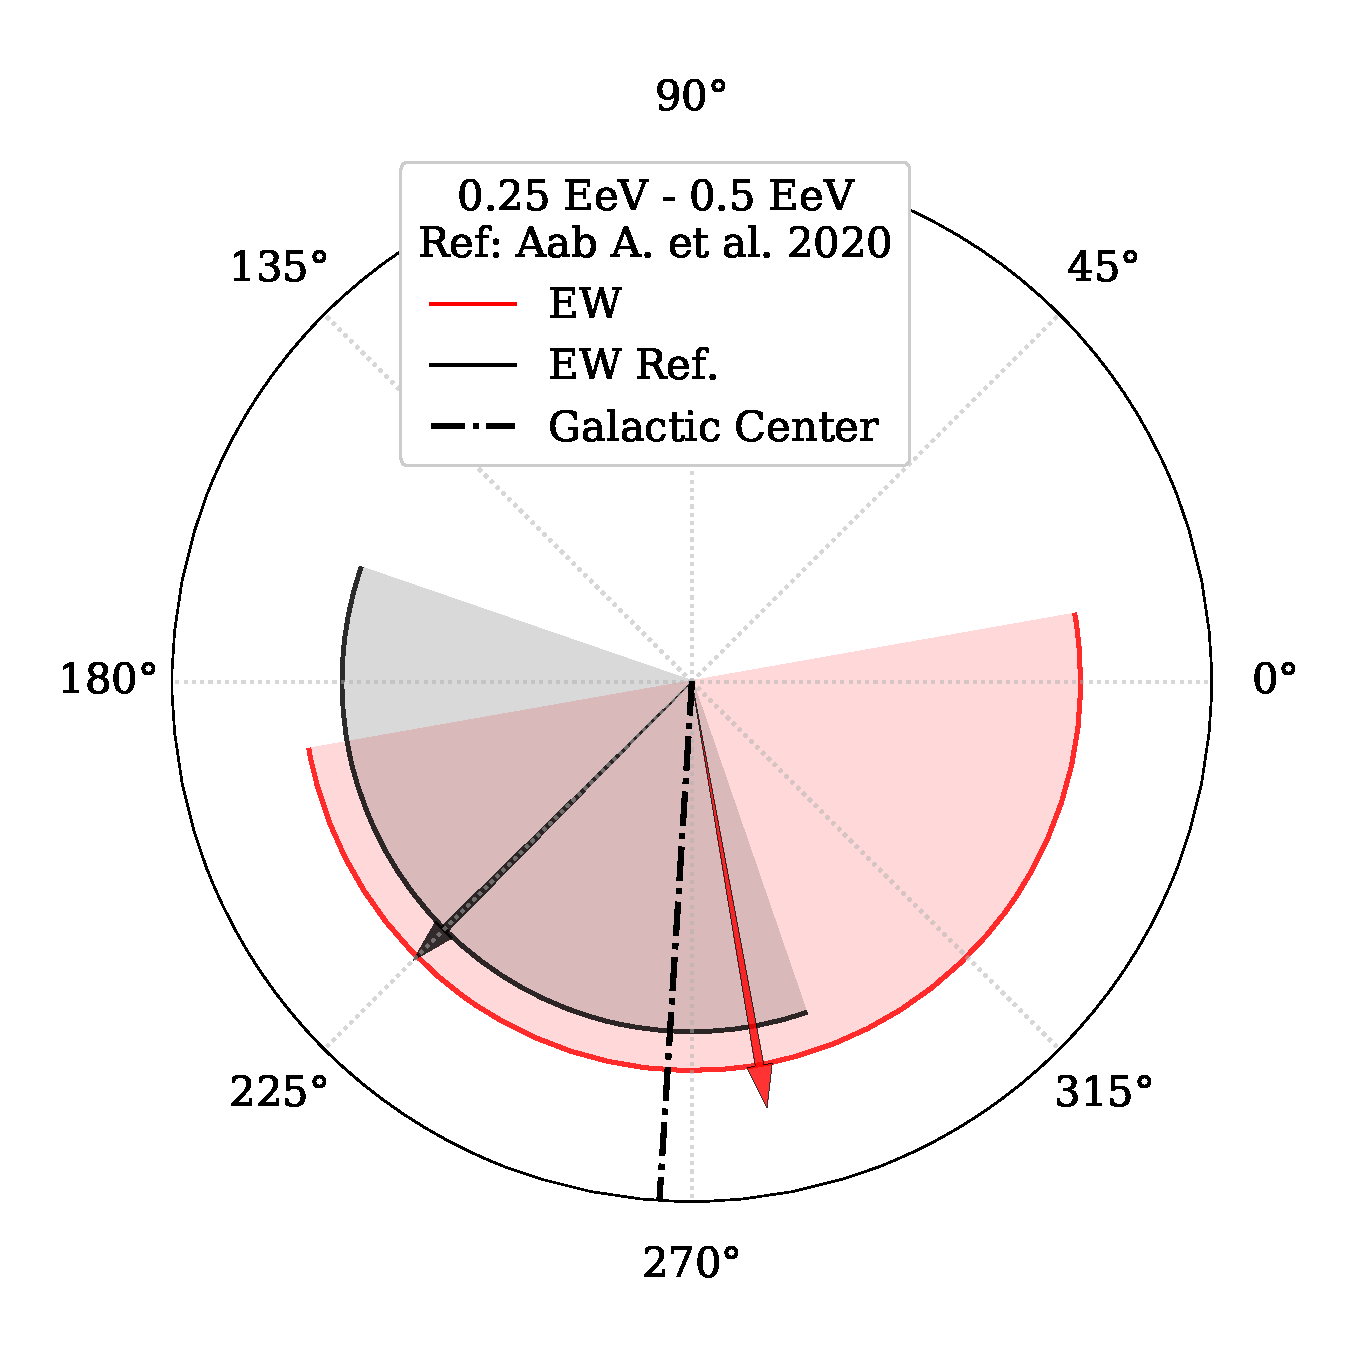
\includegraphics[width=0.65\textwidth]{Figs/phase_primer_bin_v3.pdf}
            \vspace*{-1 cm}
        \end{center}
        \caption{Valores de las fases obtenidos en este trabajo y en el trabajo Aab A. et al. (2020) \cite{Aab_2020} con sus respectivas incertidumbres para la frecuencia sidérea en el  rango 0.25 EeV - 0.5 EeV.}
        \label{fig:primer}
    \end{small}
\end{figure}


\begin{figure}[H]
    \begin{small}
        \begin{center}
            \vspace*{-0.6 cm}
            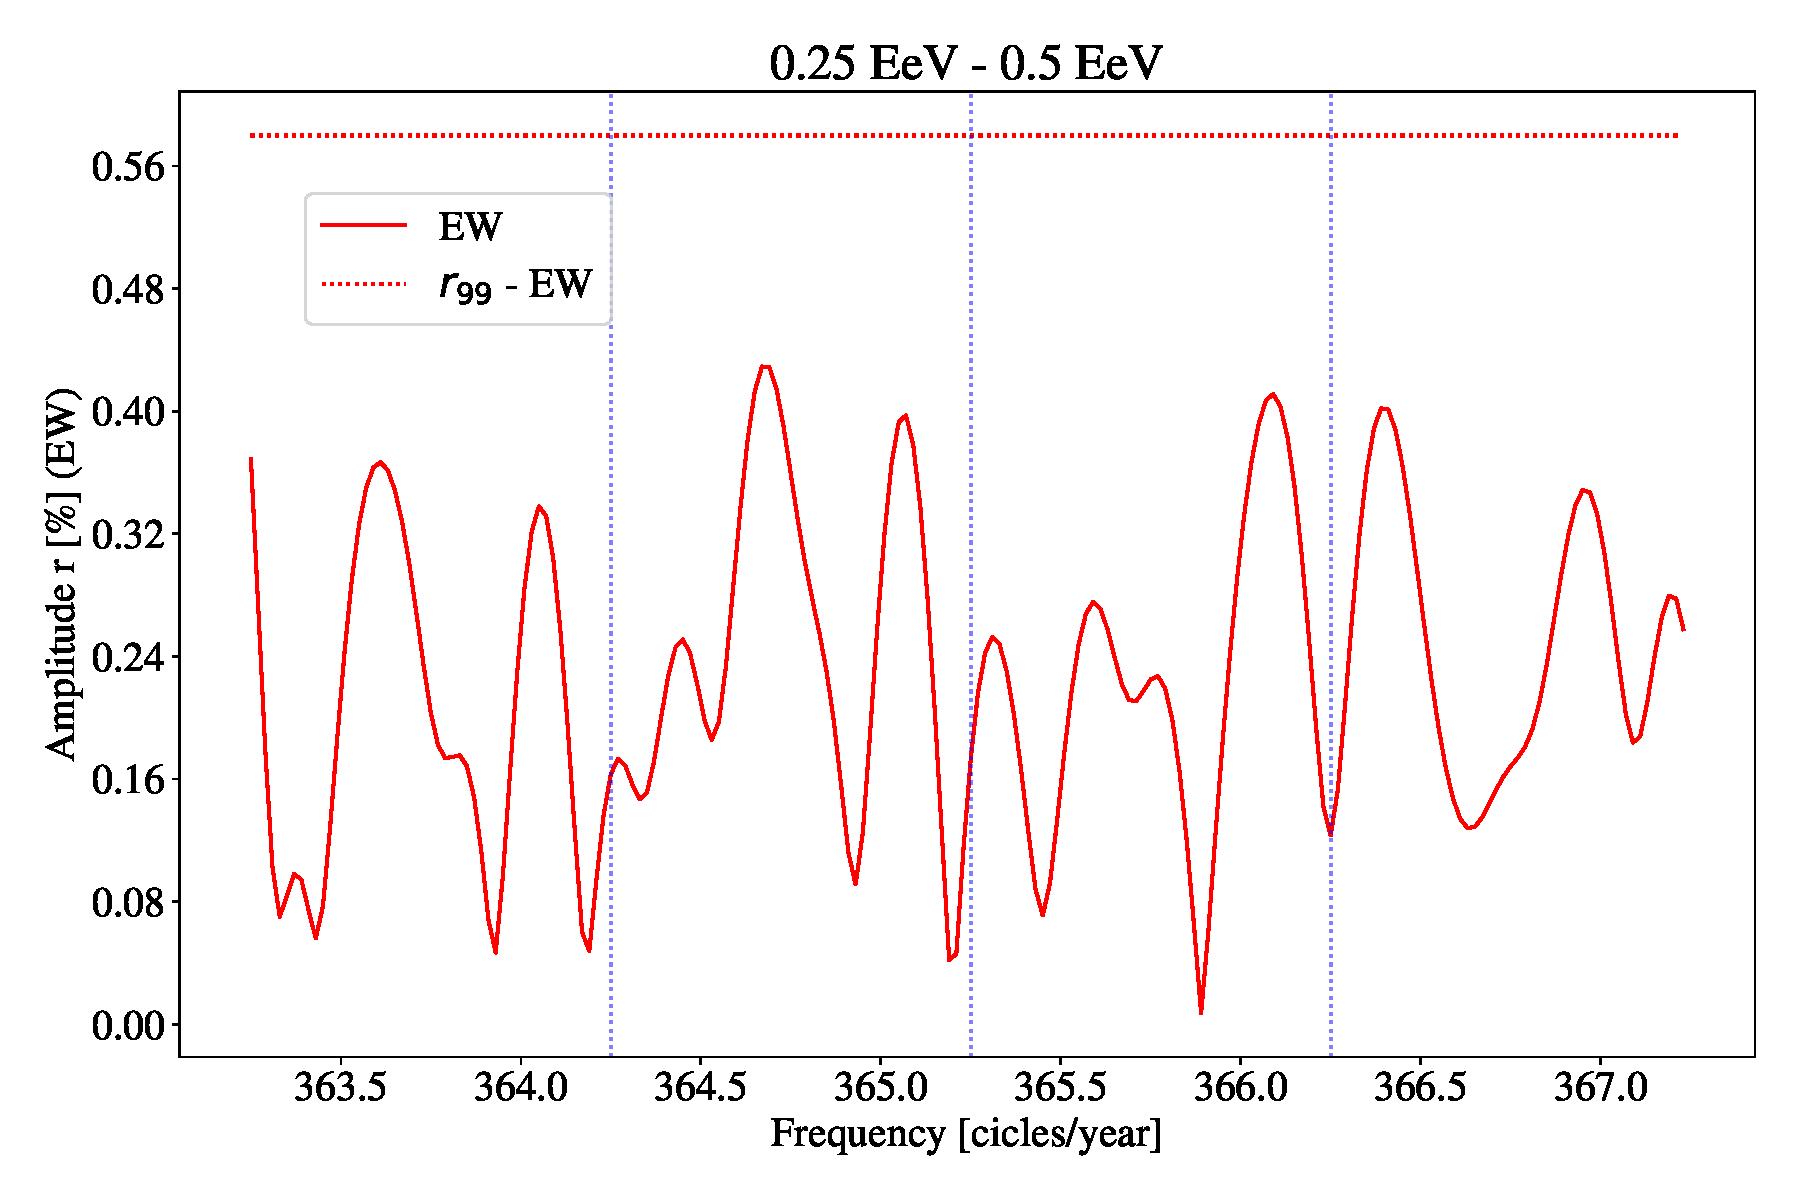
\includegraphics[width=0.9\textwidth]{Figs/plot_bin_1_barrido_v3_EW.pdf}
            \vspace*{-0.8 cm}
        \end{center}
        \caption{Barrido de frecuencias en el  rango 0.25 EeV - 0.50 EeV mediante el método East-West.}
        \label{fig:primer_barrido}
    \end{small}
\end{figure}

\subsection{Results of the 0.5 EeV - 1 EeV energy range}



\begin{table}[H]
    \begin{small}
        \begin{center}
            \begin{tabular}[c]{l|c|c||c|}
\cline{2-4}                                       & \multicolumn{2}{c||}{All Triggers}    & \multicolumn{1}{c|}{Disparo Estándar}   \\ \hline
\multicolumn{1}{|l|}{Frecuencia:                } & Solar	                & Sidérea	                & Sidérea \cite{Aab_2020}   \\ \hline
\multicolumn{1}{|l|}{Amplitude r [\%]:           } & $0.43^{+0.21}_{-0.14}$	& $0.44^{+0.21}_{-0.14}$ 	& $0.38^{+0.20}_{-0.14}$ \cite{codigo}      \\
\multicolumn{1}{|l|}{$r_{99}$ [\%]:             } & \multicolumn{2}{c||}{0.56}                          & 0.64\cite{codigo}                 \\
\multicolumn{1}{|l|}{$r^{UL}$ [\%]:             } & 0.89 	                & 0.90                      & 0.90 \cite{codigo}                 \\ 
\multicolumn{1}{|l|}{$\sigma$[\%]:              } & \multicolumn{2}{c||}{0.18}                          & 0.21 \cite{codigo}      \\\hline
\multicolumn{1}{|l|}{Amplitude $d_\perp$[\%]:    } & -	                    & $0.56^{+0.27}_{-0.18}$ 	& $0.5^{+0.3}_{-0.2}$       \\
\multicolumn{1}{|l|}{$d_{99}$ [\%]:             } & - 	                    & 0.71                      & 0.8   \cite{codigo}                \\
\multicolumn{1}{|l|}{$d_{\perp}^{UL}[\%]$       } & -                       & 1.1                       & 1.1                         \\
\multicolumn{1}{|l|}{$\sigma_{x,y}$[\%]:        } & -	                    & 0.23	                    & 0.21       \\\hline
\multicolumn{1}{|l|}{Rayleigh Probability      :        } & 0.065                   & 0.055	                    & 0.20       \\
\multicolumn{1}{|l|}{Phase[$^o$]:                } & 205$\pm$34              & 258$\pm$34                & 261$\pm$43\\ \hline
\multicolumn{1}{|l|}{$\langle\cos\delta \rangle$} & \multicolumn{2}{c||}{0.79}        	                & 0.79 \cite{codigo}        \\        
\multicolumn{1}{|l|}{$\langle\sin\theta \rangle$} & \multicolumn{2}{c||}{0.50}        	                & 0.54\cite{codigo}        \\ \hline       
            \end{tabular}
        \end{center}
    \end{small}
    \caption{Características para las frecuencias solar y sidérea con el método East-West en el primer armónico en rango de energía 0.5 EeV - 1 EeV}
    \label{tab:segundo_bin_data}
\end{table}





\begin{figure}[H]
    \begin{small}
        \begin{center}
            \vspace*{-1.6 cm}
            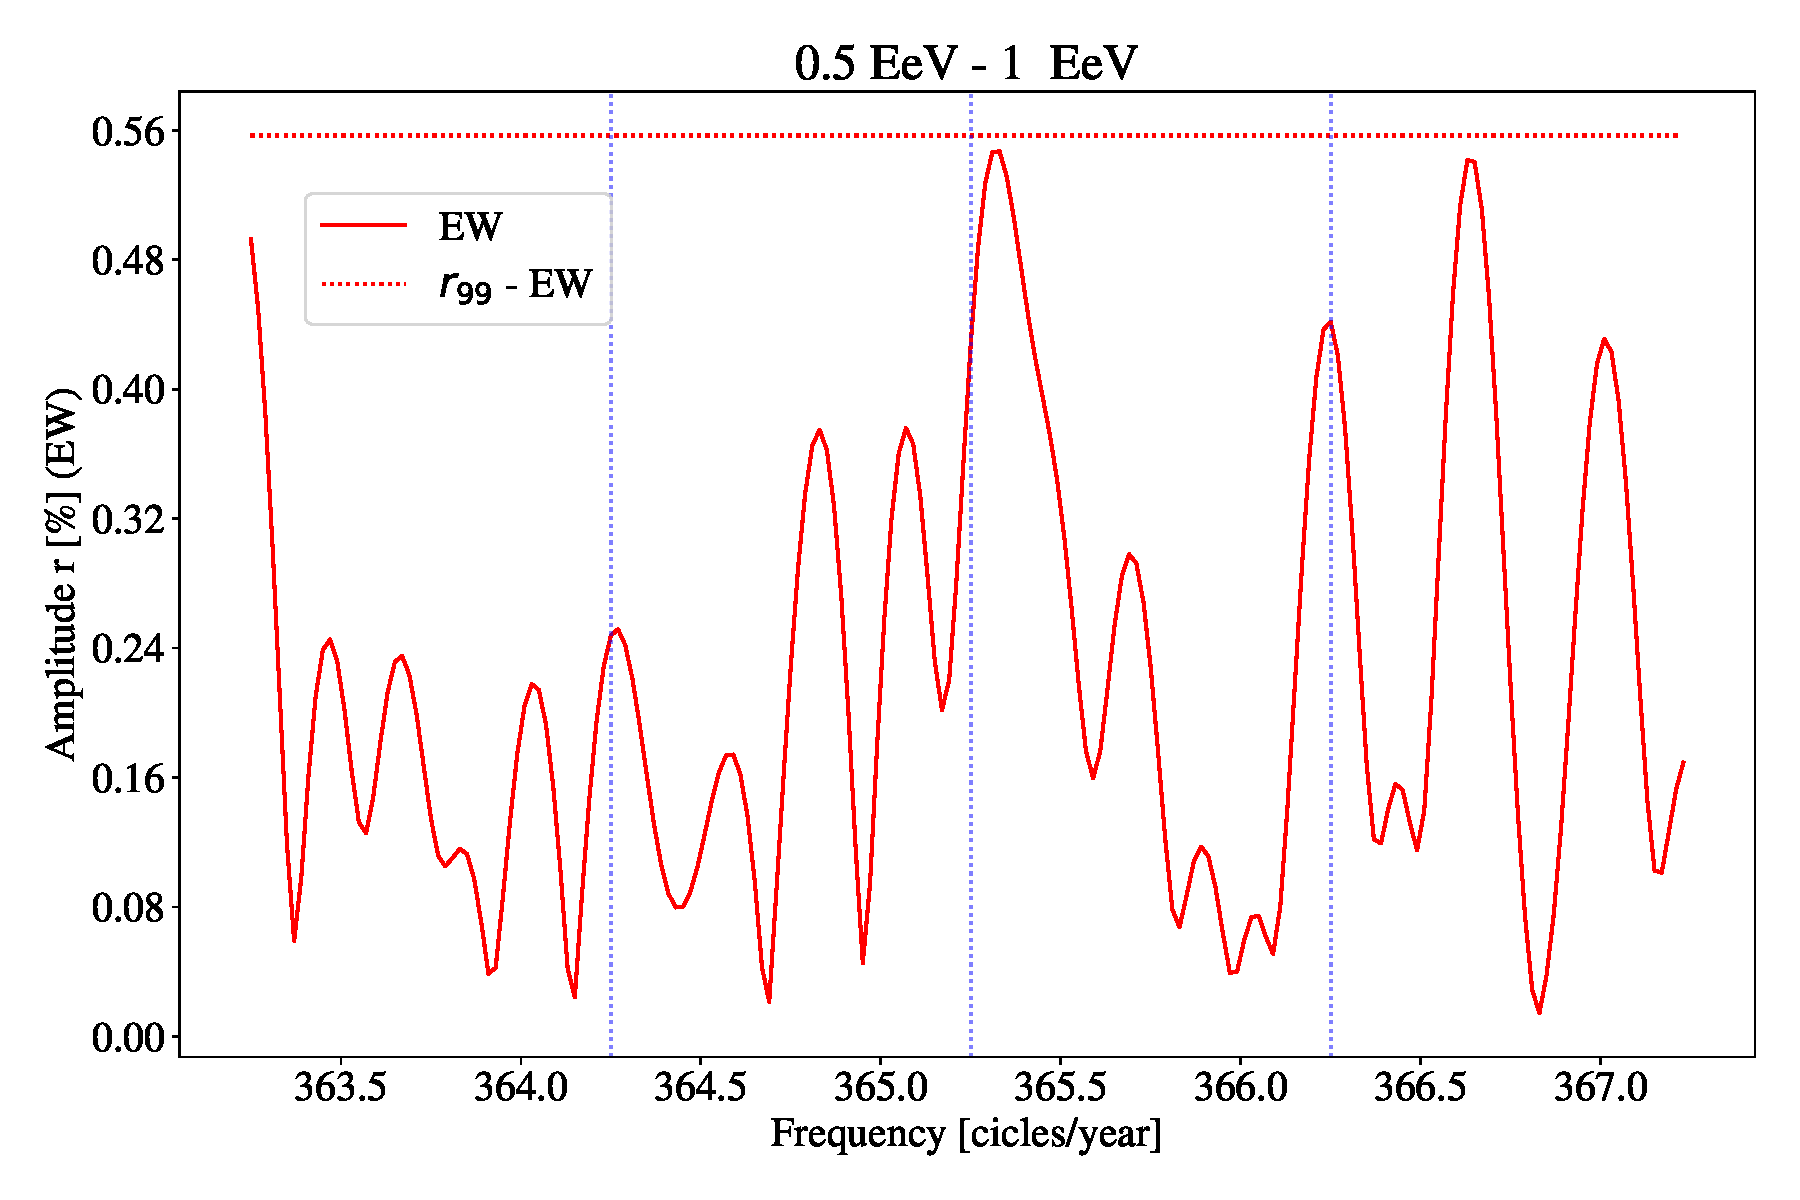
\includegraphics[width=0.9\textwidth]{Figs/plot_bin_2_barrido_v3_EW.pdf}
            \vspace*{-0.6 cm}
        \end{center}
        \caption{Barrido de frecuencias en el  rango 0.5 EeV - 1.0 EeV mediante el método East-West.}
        \label{fig:segundo_barrido}
    \end{small}
\end{figure}    


\begin{figure}[H]
    \begin{small}
        \begin{center}
            \vspace*{-0.65 cm}
            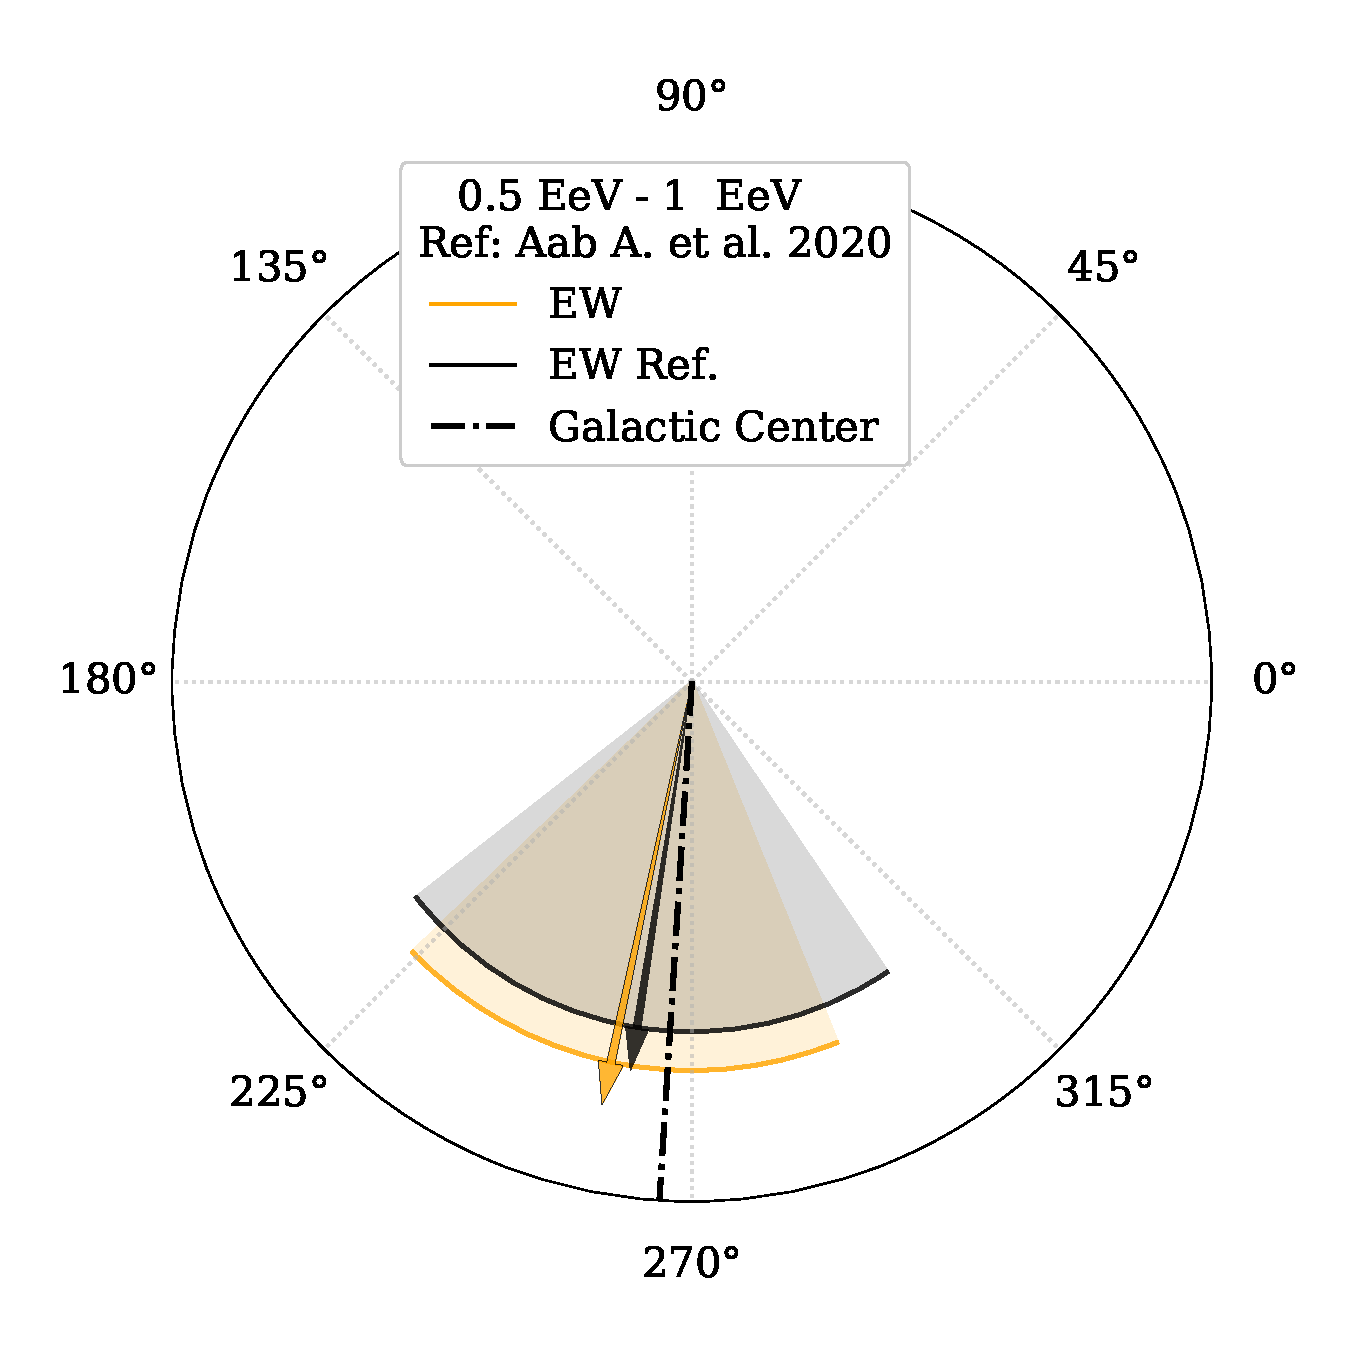
\includegraphics[width=0.65\textwidth]{Figs/phase_segundo_bin_v3.pdf}
            \vspace*{-1.1 cm}
        \end{center}
        \caption{Valores de las fases obtenidos en este trabajo y en el trabajo Aab A.  et al. (2020) \cite{Aab_2020} con sus respectivas incertidumbres para la frecuencia sidérea en el rango 0.5 EeV - 1.0 EeV .}
        \label{fig:segundo}
    \end{small}
\end{figure}


\subsection{Results of the 1 EeV - 2 EeV energy range}


\begin{table}[H]
    \begin{small}
        \begin{center}
            \begin{tabular}[c]{l|c|c|}
                \cline{2-3}         & \multicolumn{2}{c|}{Todos los disparos} \\ \cline{2-3}
                                        & Rayleigh                       & East - West            \\\hline
\multicolumn{1}{|l|}{Frecuencia:}       & \multicolumn{2}{c|}{Solar}        \\
\multicolumn{1}{|l|}{Amplitude $r$[\%]:} & $0.24^{+0.16}_{-0.09}$  & $0.28^{+0.35}_{-0.11}$ \\
\multicolumn{1}{|l|}{$r_{99}$ [\%]:   } & 0.41                    & 0.91       \\
\multicolumn{1}{|l|}{$r_{UL}$ [\%]:   } & 0.58                   & 1.1       \\
\multicolumn{1}{|l|}{$\sigma$:        } & 0.14                    & 0.30          \\\hline
\multicolumn{1}{|l|}{Rayleigh Probability:    } & 0.22                     & 0.65          \\
\multicolumn{1}{|l|}{Phase:            } & 260$\pm$48              & 279$\pm$76    \\\hline
            \end{tabular}
        \end{center}

    \end{small}
    \caption{Características para la frecuencia solar con los métodos de Rayleigh  e East-West en el primer armónico en el rango 1 EeV - 2 EeV.}
    \label{tab:solar_3}
\end{table}


\begin{figure}[H]
    \begin{small}
        \begin{center}
            
            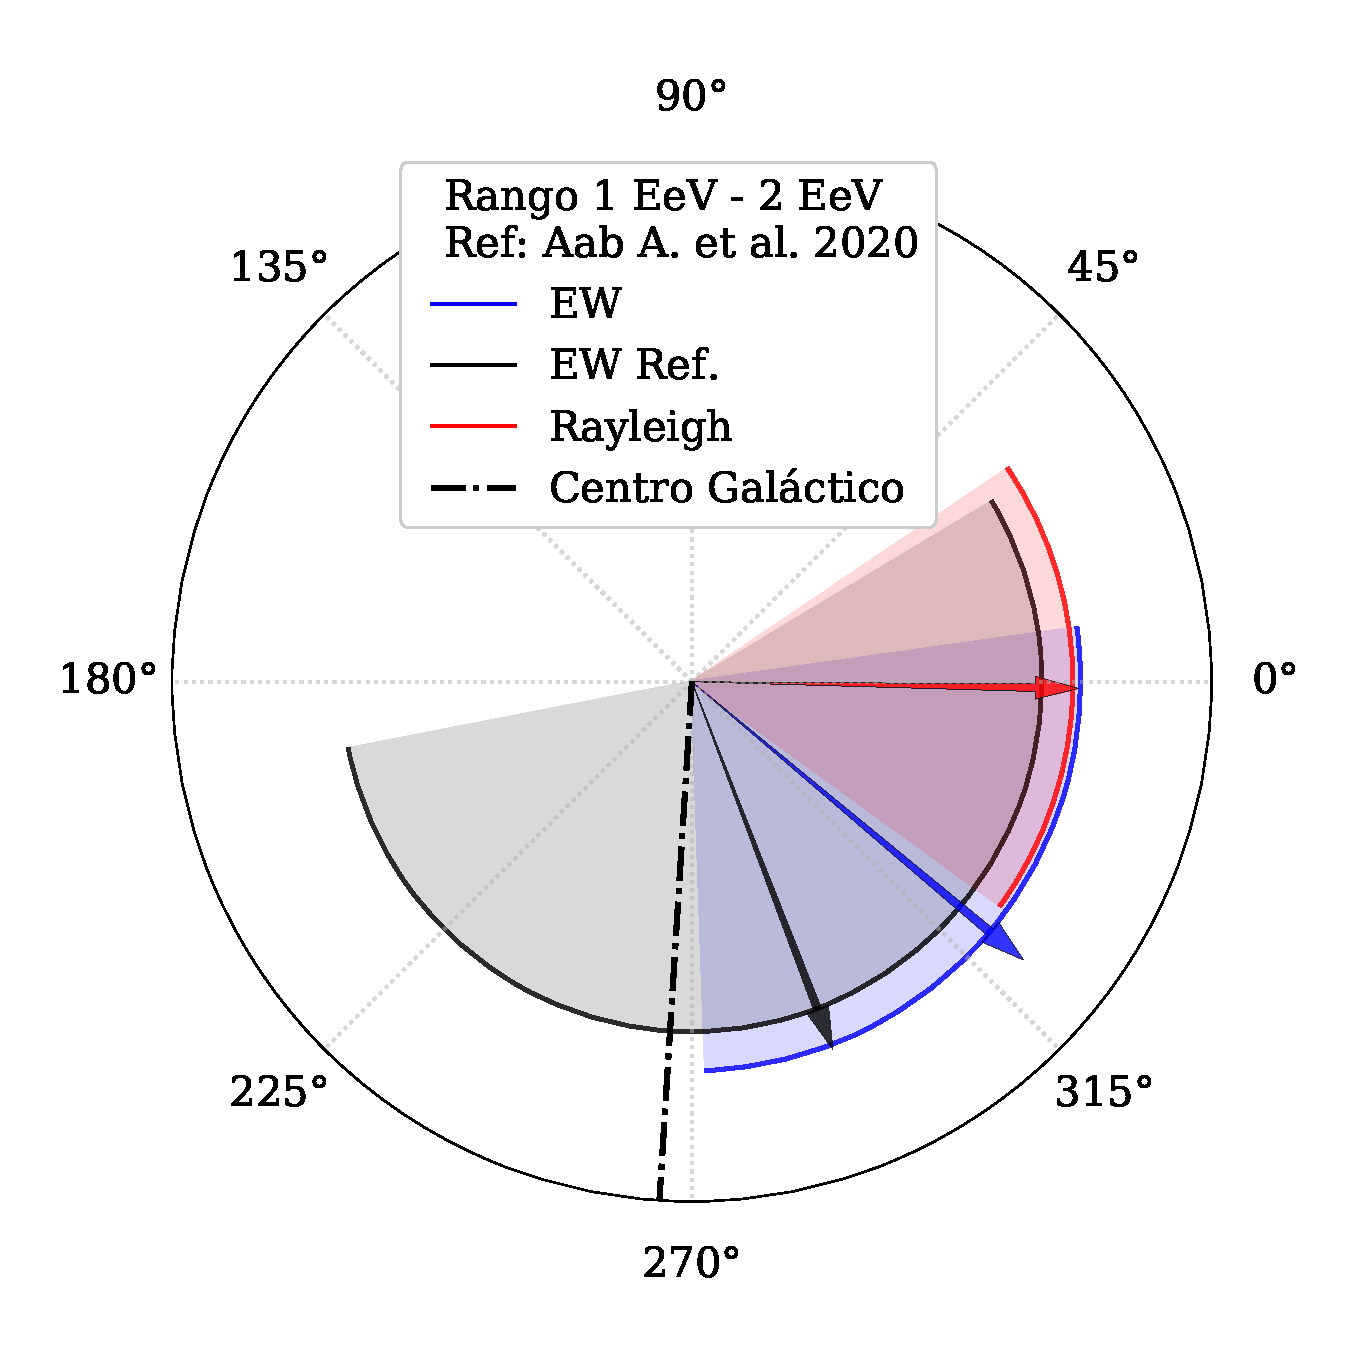
\includegraphics[width=0.65\textwidth]{Figs/phase_tercer_bin_v3.pdf}
            \vspace*{-1.2 cm}
        \end{center}
    \caption{Valores de las fases obtenidos en este trabajo y en el trabajo Aab A. et al. (2020) \cite{Aab_2020} con sus respectivas incertidumbres para la frecuencia sidérea en el  rango 1.0 EeV - 2.0 EeV .}
    \label{fig:tercer}
    \end{small}
\end{figure}
\begin{table}[H]
    \vspace*{-0.51 cm}
    \begin{small}
        \begin{center}
            \begin{tabular}[c]{l|c|c||c|}
                \cline{2-4}                 & \multicolumn{2}{c||}{All Triggers}                  & Disparo Estándar      \\
                \cline{2-4}                 & Rayleigh                          & East - West                 & East - West\cite{Aab_2020}      \\\hline
\multicolumn{1}{|l|}{Frecuencia:             }  & \multicolumn{2}{c||}{Sidérea}                               & Sidérea        \\ \hline
\multicolumn{1}{|l|}{Amplitude $r$ [\%]:      }  & $0.32^{+0.16}_{-0.10}$ 	    & $0.5^{+0.3}_{-0.2}$         & $0.14^{+0.37}_{-0.02}$\cite{codigo}       \\
\multicolumn{1}{|l|}{$r_{99}$[\%]:           }  & 0.41	                        & 0.91                        & 0.84\cite{codigo}        \\
\multicolumn{1}{|l|}{$r^{UL}[\%]$      }        & 0.66                          & 1.3                         & 0.89 \cite{codigo}        \\
\multicolumn{1}{|l|}{$\sigma$[\%]:     }        & 0.14                          & 0.30	                    & 0.28 \cite{codigo}          \\ \hline
\multicolumn{1}{|l|}{Amplitude $d_\perp$ [\%]:}  & $0.41^{+0.20}_{-0.13}$        & $0.6^{+0.4}_{-0.3}$         & $0.18^{+0.47}_{-0.02}$       \\ 
\multicolumn{1}{|l|}{$d_{99}$[\%]:           }  & 0.53	                       & 1.1                         & 1.1\cite{codigo}        \\
\multicolumn{1}{|l|}{$d_{\perp}^{UL}[\%]$    }  & 0.84                          & 1.6                         & 1.1        \\
\multicolumn{1}{|l|}{$\sigma_{x,y}$[\%]:     }  & 0.17                          & 0.38	                    & 0.35          \\ \hline
\multicolumn{1}{|l|}{Rayleigh Probability:           }  & 0.063	                           & 0.26                        & 0.87          \\
\multicolumn{1}{|l|}{Phase[$^o$]:             }  & 357$\pm$35                   & 320$\pm$48                 & 291$\pm$100      \\\hline
\multicolumn{1}{|l|}{$\langle\cos\delta\rangle$}&{0.78}                               & 0.78       \\        
\multicolumn{1}{|l|}{$\langle\sin\theta\rangle$}&{0.55}                               & 0.57       \\ \hline       
\end{tabular}
        \end{center}
    \end{small}
    \vspace*{-0.21 cm}
    \caption{Características para la frecuencia sidérea con los métodos de Rayleigh  e East-West en el primer armónico en el rango 1 EeV - 2 EeV.}
    \label{tab:siderea_3}
\end{table}



\begin{figure}[H]
    \begin{small}
        \begin{center}
            
            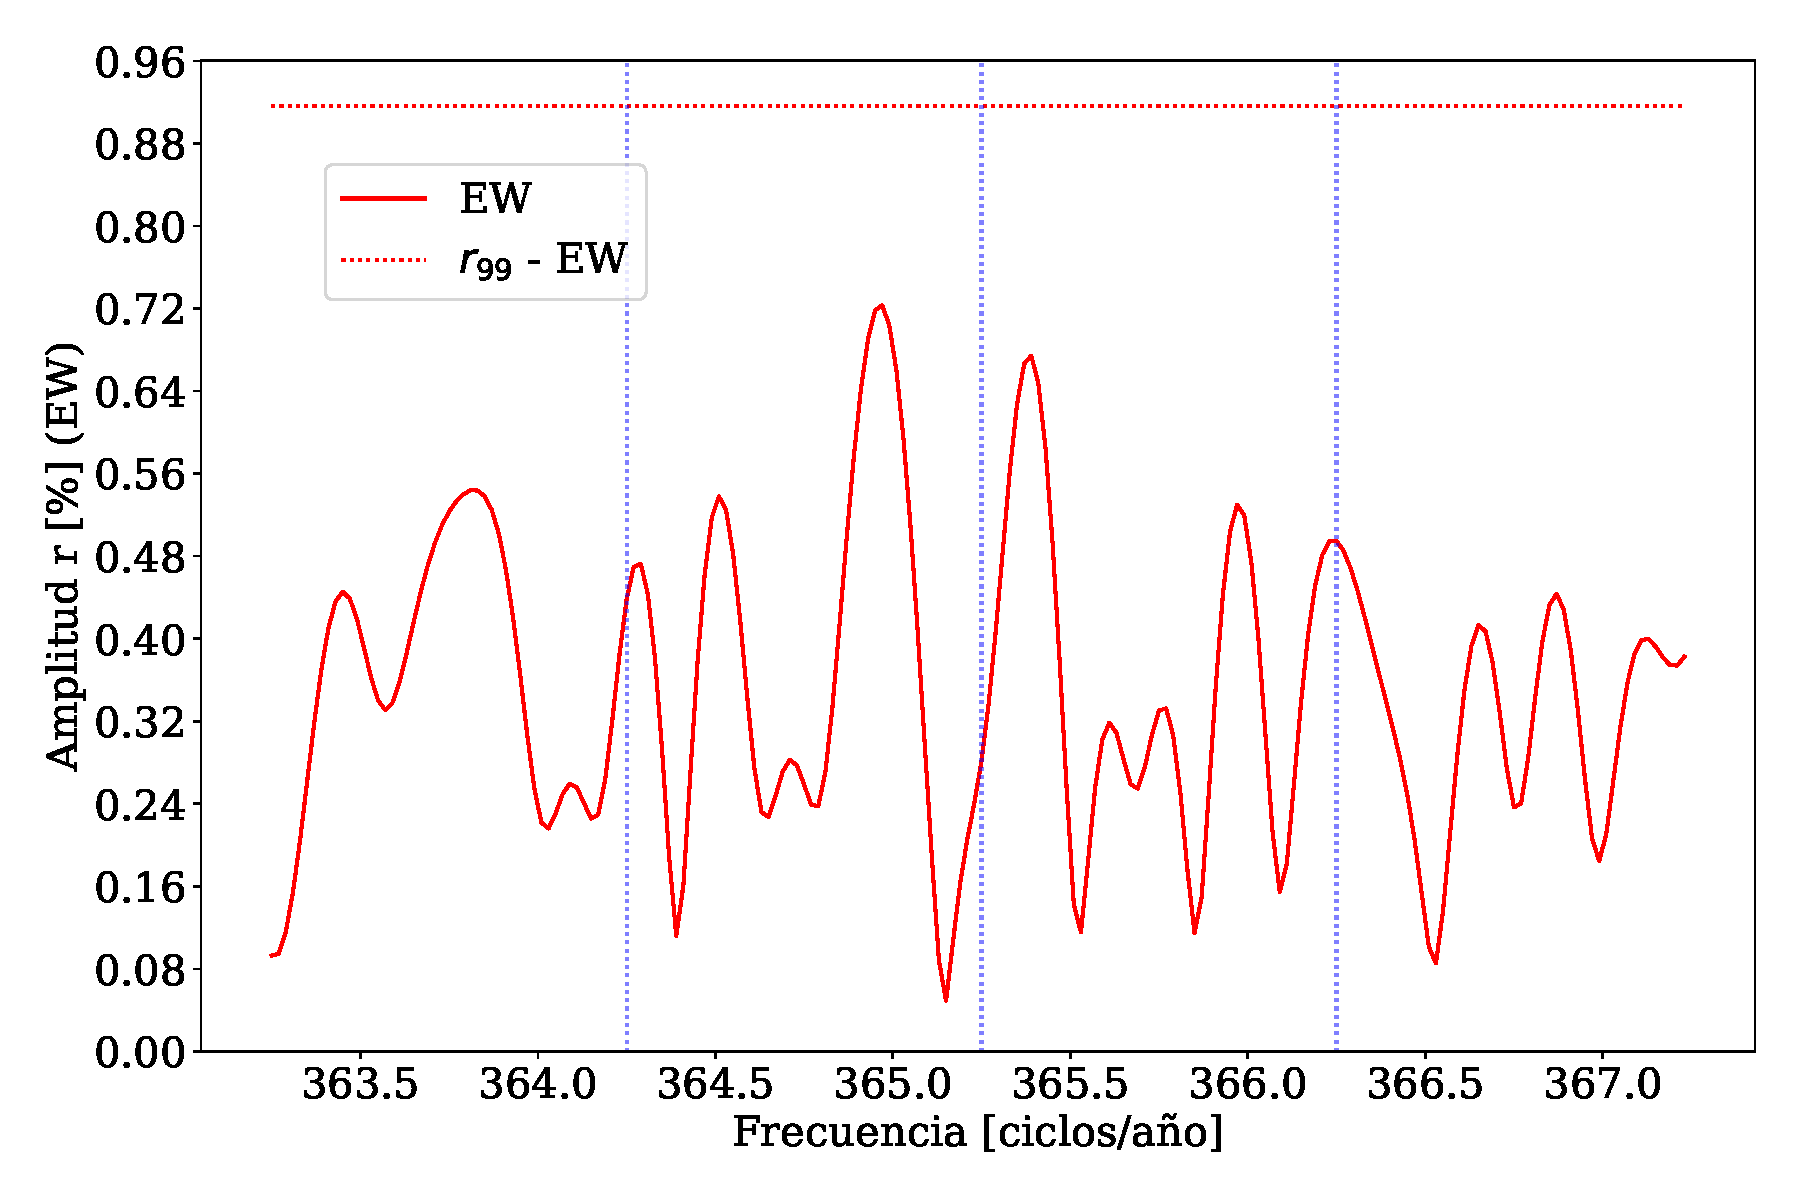
\includegraphics[width=0.9\textwidth]{Figs/plot_bin_3_barrido_v3_EW.pdf}
            \vspace*{-1 cm}
        \end{center}
        \caption{Barrido de frecuencias en el rango 1 EeV - 2 EeV mediante el método East-West.}
        \label{fig:tercer_barrido}
    \end{small}
\end{figure}    

\section{Análisis de los resultados}

\begin{figure}[H]
    \begin{small}
        \begin{center}
            
            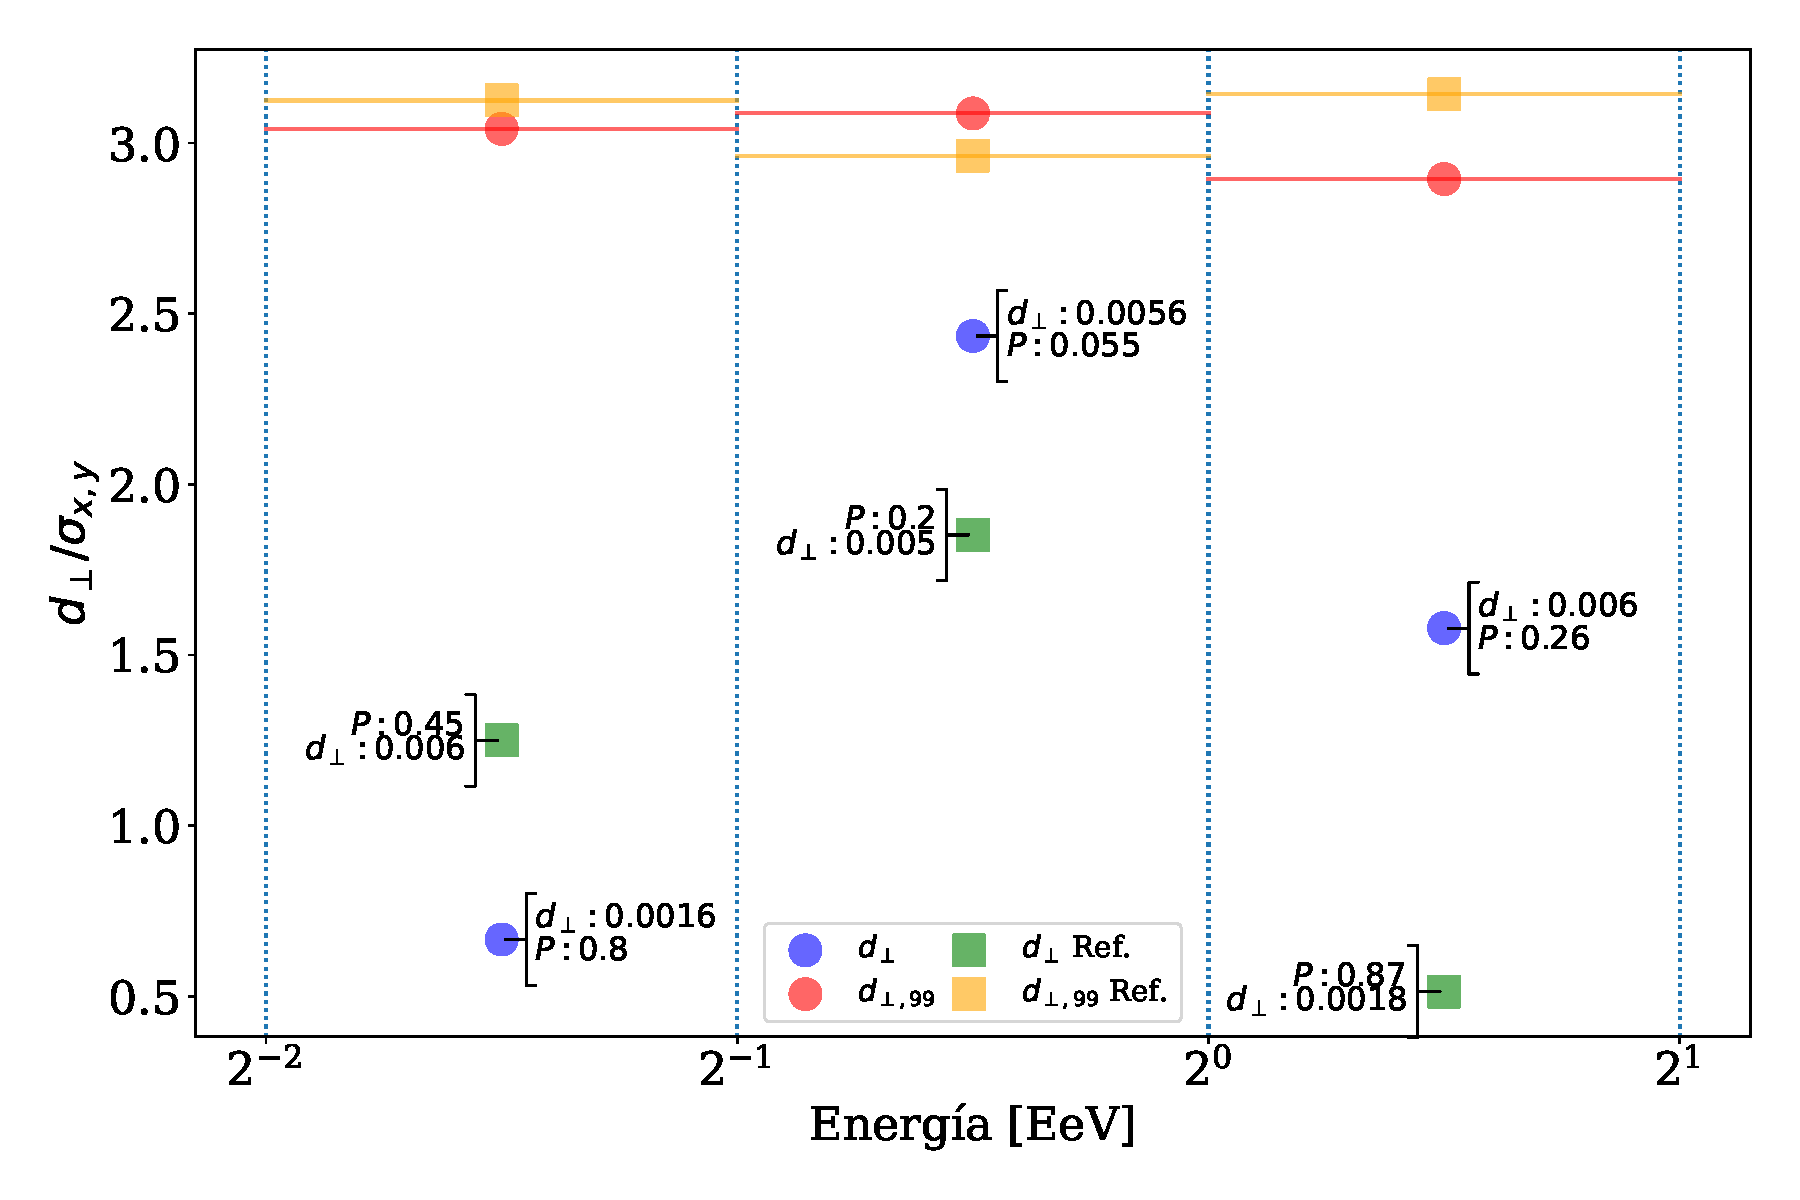
\includegraphics[width=\textwidth]{Figs/d_perp_normalizado_sigmas_v6.pdf}
            \vspace*{-1 cm}
        \end{center}
        \caption{Variaciones de la amplitud $d_\perp$ con respecto a $\sigma_{x,y}$ comparados con $d_{\perp,99}$ para distintos rangos de energía. Estos valores son obtenidos con el método East-West. }
        \label{fig:normalizado_sigma}
    \end{small}
\end{figure}

\begin{figure}[H]
    \begin{small}
        \begin{center}
            
            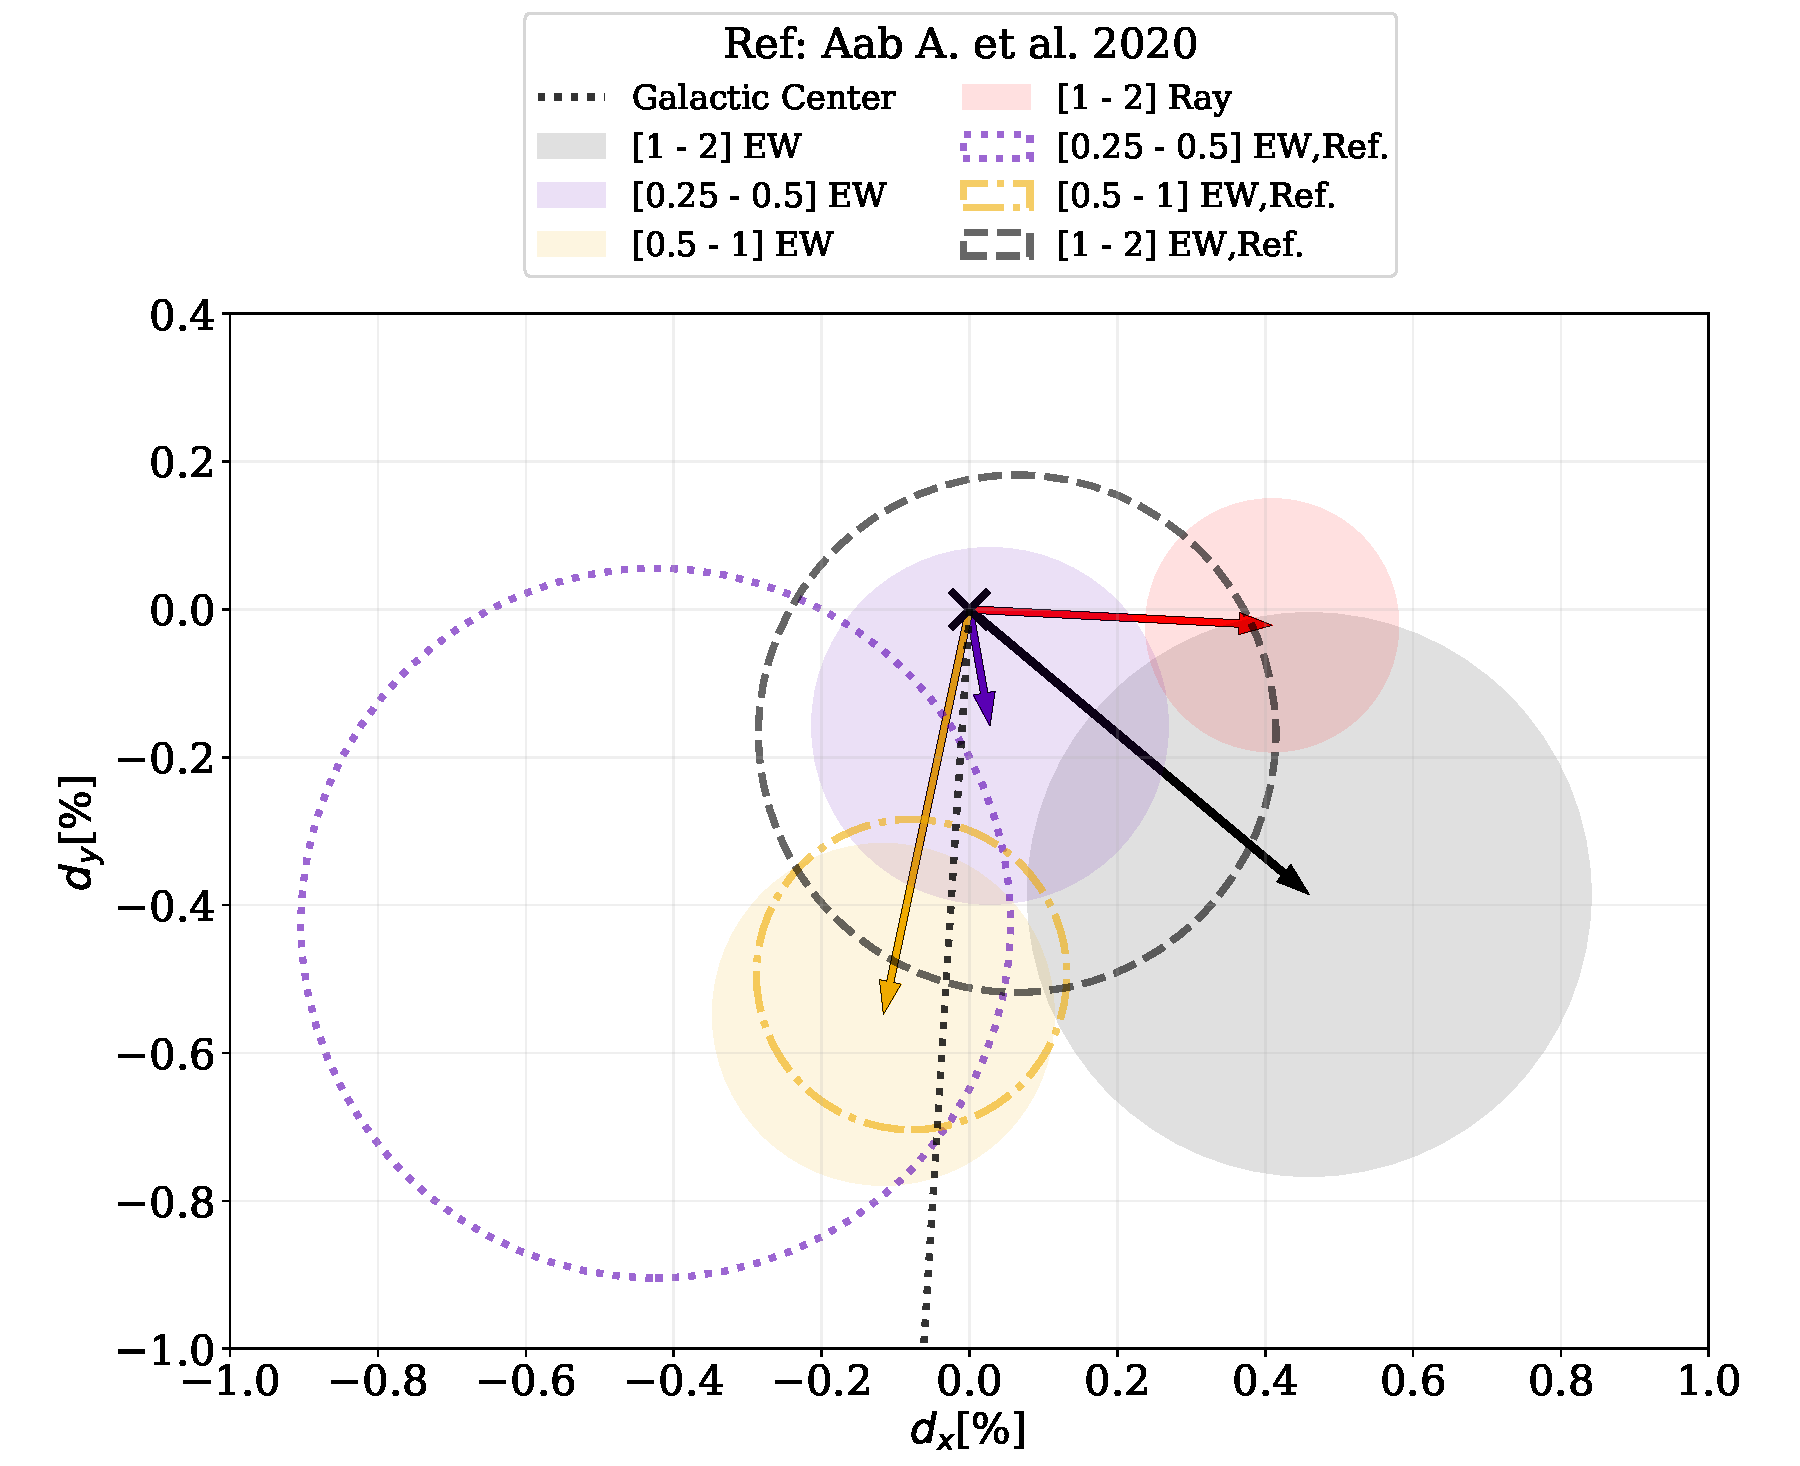
\includegraphics[width=\textwidth]{Figs/comparando_sigmas_v4.pdf}
            \vspace*{-1. cm}
        \end{center}
        \caption{Amplitudes con incertidumbre, apuntando en la dirección  de la fase. Los círculos punteados los valores del trabajo Aab A. et al. (2020) \cite{Aab_2020} con sus respectivas incertidumbres y la línea punteada en negro marca la dirección del centro galáctico.}
        \label{fig:incertidumbre}
    \end{small}
\end{figure}

\begin{thebibliography}{9}
    \bibitem{Aab_2020}
    {Aab A. et al.},{Cosmic-Ray Anisotropies in Right Ascension Measured by the {Pierre   Auger Observatory}}.
    \emph{The Astrophysical Journal}, \textbf{891}~(2), 142, 2020. \url{https://doi.org/10.3847/1538-4357/ab7236}.
\end{thebibliography}
    

\end{document}